% Utilities and Experimental Suites
\clearpage
\chapter{Utilities and Experimental Suites}
Outside the core modules, such as the data recorder, RTXI provides a number of useful utilities and experimental suites. While most utilities are designed as an optional aid, RTXI has a growing library of experimental suites intended to perform complete biological experiments. The experimental suites can be augmented with user-written custom modules to create complex experimental systems outside the intended use of these suites. For RTXI version 1.4, the Patch Clamp Experimental Suite is the only suite currently available. However, a number of other suites, such as a digital camera and imaging suite, are in construction.

% Signals
\clearpage
\section{Signal Utilities}
The signal utilities are modules that can output several types of standard signals. These modules are useful for diagnostic purposes, such as testing a data acquisition board, or can be used as part of an experimental protocol, such as white noise injection into a neuronal network.

\subsection{Signal Generator}
%Signal Generator Module

\subsubsection{Overview}
\label{Signal Generator}
\index{Signal Generator}\index{utilities, Signal Generator}

\begin{figure}[h]
\begin{center}
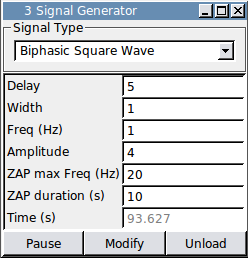
\includegraphics[width=2in]{siggen-tutorial1.png} 
\caption[Signal Generator]{The signal generator module is set to output a 1s long biphasic square wave every 5s, with an amplitude of 4. A tutorial is provided to replicate this figure.}
\end{center}
\label{siggen1}
\end{figure}

The signal generator module can generate a number of different signals, and each signal is modified through several parameters. The available signals and their corresponding parameters are described below.

\begin{itemize}
\item Sine Wave: requires frequency and amplitude
\item Monophasic Square Wave: requires delay, pulse width, and pulse amplitude
\item Biphasic Square Wave: requires delay, pulse width, and pulse amplitude
\item Sawtooth Wave: requires delay, pulse width, and maximum amplitude
\item ZAP Stimulus: needs starting and ending frequencies, amplitude, and duration of ZAP
\end{itemize}

All signals are continuous except for the ZAP stimulus, which has a specified duration.

\subsubsection{Output Channels}
\begin{description}
\item [Signal Waveform]Signal output
\end{description}

\subsubsection{Parameters}
\begin{description}
\item [Delay (s)]Time before each square wave or sawtooth wave starts
\item [Width (s)]Width of each square wave and sawtooth signal
\item [Freq (Hz)]frequency of sine wave and starting frequency for ZAP stimulus
\item [Amplitude]amplitude for all signals
\item [ZAP max Freq (Hz)]maximum frequency for ZAP stimulus
\item [ZAP duration (s)]duration of ZAP stimulus
\end{description}

\subsubsection{Tutorial}
\label{siggen tutorial}\index{Signal Generator, tutorial}\index{tutorial, Signal Generator}
In this tutorial, the Signal Generator will be used to output a biphasic square wave every 5s. Each phase will be 1s long, with an amplitude of 4. The oscilloscope will be used to visualize the signal, with the option of outputting the signal through a data acquisition board. The mimic tutorial continues where this tutorial leaves off,\seealso{Chapter \ref{mimic tutorial}\\Mimic Tutorial} so it is suggested that is done next.

\begin{enumerate}
\item Open the Signal Generator module through the menu: \textbf{Utilities}$\rightarrow$\textbf{Signals}$\rightarrow$\textbf{Signal Generator}
\item Open the oscilloscope module through the menu: \textbf{System}$\rightarrow$\seealso{Chapter \ref{Oscilloscope}\\Oscilloscope}\textbf{Oscilloscope}
\item Set the correct parameters for the desired biphasic square wave in the signal generator GUI as in Figure \ref{siggen1}:
  \begin{itemize}
  \item Set the signal type to \textbf{Biphasic Square Wave} using the pull down menu under \textbf{Signal Type}
  \item To output the signal every 5s, set \textbf{Delay} to 5
  \item To set each phase to be 1s long, set \textbf{Width} to 1
  \item To set the amplitude to 4V, set \textbf{Amplitude} to 4
  \item Save changes by clicking the \textbf{Modify} button
  \end{itemize}
\item Set up the oscilloscope to visualize the signal by right clicking on the oscilloscope and selecting \textbf{Properties}
  \begin{itemize}
  \item Make sure the \textbf{Channel} Tab is currently selected
  \item Select \textbf{Signal Generator} under the channel pulldown menu (This probably will already be selected)
  \item Select \textbf{Output} in the following pulldown menu on the right
  \item Select \textbf{Signal Waveform} in the following pulldown menu on the right (This probably will already be selected)
  \item Activate this channel by hitting the toggle button \textbf{Active}
  \item Change the scale to \textbf{1 V/div} in the Scale pulldown menu
  \item Click the \textbf{Apply} button to save the changes
  \item Select the \textbf{Display} tab
  \item Change the time scale to \textbf{1 s/div}
  \item Change the refresh rate to 50 for a smoother looking output
  \item Click the \textbf{Apply} button to save the changes
  \end{itemize}
\item \textit{Optional} Output the signal generator signal through the analog output of a data acquisition board
  \begin{itemize}
  \item Open the connector module through the menu: \textbf{System}$\rightarrow$\textbf{Connector}
  \item In the Output Block, select \textbf{Signal Generator} under block and \textbf{Signal Waveform} under Channel
  \item In the Input Block, select your data acquisition board (i.e. /dev/comedi0 or NI-PCI6259) and the desired channel (i.e. Analog Output 0)
  \item Connect the two by toggling the arrow button
  \item Make sure the desired channel is active through the \seealso{Chapter \ref{system control panel}\\System Control Panel}System Control Panel
  \end{itemize}
\item Start the signal by untoggling the \textbf{Pause} button
\item The biphasic square wave should now be seen on the oscilloscope as in Figure \ref{siggen1}
\end{enumerate}

\begin{figure}[h]
\begin{center}
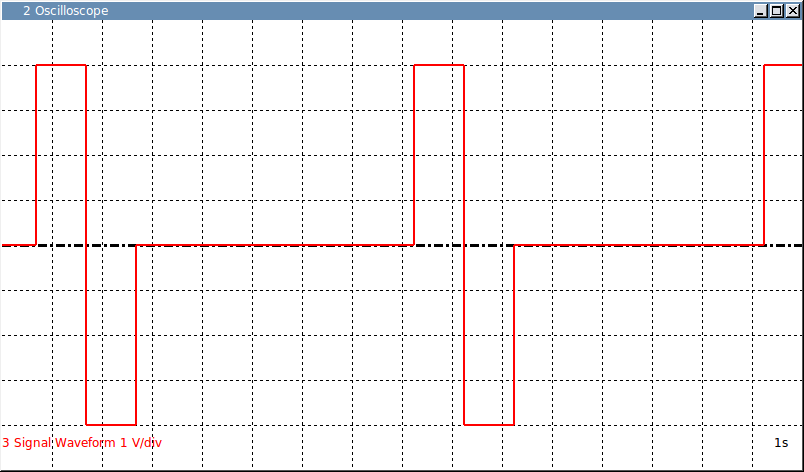
\includegraphics[width=4.5in]{siggen-tutorial2.png} 
\caption[Signal Generator Output]{The oscilloscope is used to visualize a biphasic square wave being output by the Signal Generator Module} 
\end{center}
\label{siggen2}
\end{figure}

\subsection{Mimic}
%Mimic Module

\subsubsection{Overview}
\label{Mimic}
\index{Mimic}\index{utilities, Mimic}

\begin{figure}[h]
\begin{center}
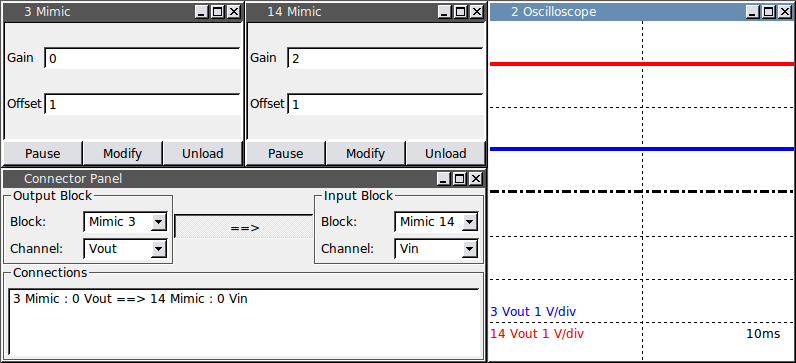
\includegraphics[width=4.5in]{mimic.png} 
\caption[Mimic]{Two Mimic modules are connected with their outputs displayed on the oscilloscope. Mimic-3, as shown in the blue oscilloscope trace, is outputting an offset of 1. As shown in the connector, Mimic-3's output (Vout) is connected to Mimic-14's (Vin). Mimic-14 applies the set gain and offset to Mimic-3's signal (1*2+1), resulting in an output of 4 shown in red. A tutorial is provided to replicate this figure.}
\end{center}
\label{mimic1}
\end{figure}

The Mimic module is the simplest signal generator available in RTXI. Mimic's main function is to apply a gain and/or offset to a signal it receives. By itself, Mimic can also be used output a continuous signal.

\subsubsection{Input Channels}
\begin{description}
\item [Vin]Gain and offset applied to this input to calculate output
\end{description}

\subsubsection{Output Channels}
\begin{description}
\item [Vout]Output calculated by multiplying input signal by gain and adding offset
\end{description}

\subsubsection{Parameters}
\begin{description}
\item [Gain]Factor by which input is multiplied
\item [Offset]Factor added to the input. If no input is connected (i.e. input = 0), offset solely determines output
\end{description}

\subsubsection{Tutorial}
\label{mimic tutorial}\index{Mimic, tutorial}\index{tutorial, Mimic}
This tutorial is meant to be performed after the Signal Generator tutorial. The mimic module will be used to add a gain of 0.5 and offset of 1 to the biphasic square wave output by the signal generator.

\begin{enumerate}
\item Use the signal generator to output a biphasic square wave, where each phase is 1s long and has an amplitude of 4. Output this signal to the oscilloscope. These steps are covered in the Signal Generator tutorial. \seealso{Chapter \ref{siggen tutorial}\\Signal Generator Tutorial}
\item Open up a Mimic module through the menu: \textbf{Utilities}$\rightarrow$\textbf{Signals}$\rightarrow$\textbf{Mimic}
\item Open the Connetor Panel through the menu: \textbf{System}$\rightarrow$\seealso{Chapter\ref{Connector}\\Connector}\textbf{Connector}
\item Connect the output of the Signal Generator module to the input of Mimic
  \begin{itemize}
  \item In the output block on the left side of the \textbf{Connector Panel}, select the Signal Generator module. The channel option should default to its only option, \textbf{Signal Waveform}
  \item In the input block on the right side of the \textbf{Connector Panel}, select the other Mimic module. The channel option should default to its only option, \textbf{Vin}
  \end{itemize}
\item Set up the oscilloscope to visualize the output of the Mimic module, in conjunction with the output of Signal Generator,  by right clicking on the oscilloscope and selecting \textbf{Properties}
  \begin{itemize}
  \item Make sure the \textbf{Channel} Tab is currently selected
  \item Select the Mimic module under the channel pulldown menu
  \item Select \textbf{Output} in the following pulldown menu, and make sure \textbf{Vout} is the selected output
  \item Activate the channel by hitting the toggle button \textbf{Active}
  \item Change the scale to \textbf{1 V/div} in the Scale pulldown menu
  \item Change the color to \textbf{Blue}
  \item Click the \textbf{Apply} button to save the changes
  \end{itemize}
\item Set the \textbf{Gain to 2} and the \textbf{Offset} to 1
\item Untoggle the \textbf{Pause} button
\item The output should now appear on the oscilloscope as in Figure \ref{mimic2}
\end{enumerate}

\begin{figure}[h]
\begin{center}
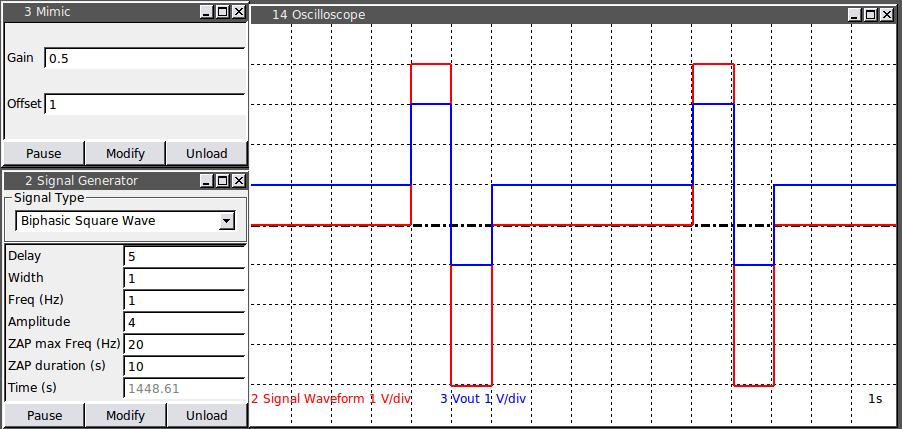
\includegraphics[width=4.5in]{mimic2.png} 
\caption[Mimic]{The Signal Generator module is outputting a biphasic square wave (red trace). This output is connected to the input of the Mimic module. The mimic module is applying a gain of 0.5 and an offset of 1 to the biphasic square, and outputs this modified signal (blue trace).}
\end{center}
\label{mimic2}
\end{figure}

\subsection{Noise Generator}
%Noise Generator Module

\subsubsection{Overview}
\label{Noise Generator}
\index{Noise Generator}\index{utilities, Noise Generator}

\begin{figure}[h]
\begin{center}
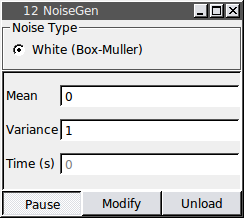
\includegraphics[width=2in]{noisegen.png} 
\caption[Noise Generator]{The noise generator module outputs Gaussian white noise.} 
\end{center}
\label{wavemaker}
\end{figure}

The noise generator module can continuously generate Gaussian white noise computed using the Box-Muller method.

\subsubsection{Output Channels}
\begin{description}
\item [Noise Waveform]Noise output
\end{description}

\subsubsection{Parameters}
\begin{description}
\item [Mean]Mean value of noise output
\item [Variance]The given variance used in noise calculated
\end{description}

\subsection{Wave Maker}
%Wave Maker Module

\subsubsection{Overview}
\label{Wave Maker}
\index{Wave Maker}\index{utilities, Wave Maker}

\begin{figure}[h]
\begin{center}
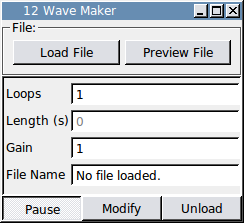
\includegraphics[width=2in]{wavemaker.png} 
\caption[Wave Maker]{The wave maker module allows the output of a pre-recorded signal from an ASCII file.} 
\end{center}
\label{wavemaker}
\end{figure}

The wavemaker module loads data from an ASCII formatted file. It samples one value from the file on every time step and generates an output signal. The module computes the time length of the waeform based on the current real-time period, set through the (\seealso{Chapter \ref{system control panel} \\System Control Panel}System Control Panel. User-generated modules can be tested using the wavemaker module, by simulating real-time acquisition of data.

\subsubsection{Output Channels}
\begin{description}
\item [Output]Values read from the ASCII file
\end{description}

\subsubsection{Parameters}
\begin{description}
\item [Loops]Number of times to repeat the waveform, looping back to the beginning
\item [Gain]Multiplicative gain to apply to the waveform values
\end{description}

% Filters
\clearpage
\section{Filter Utilities}
RTXI provides modules to filter incoming signal, which are most commonly used for analog signals received through a data acquisition board. 

\subsection{FIR Filter}
%FIR Filter Module

\subsubsection{Overview}
\label{FIR Filter}
\index{FIR Filter}\index{utilities, FIR Filter}\index{filter, FIR Filter}

\begin{figure}[h]
\begin{center}
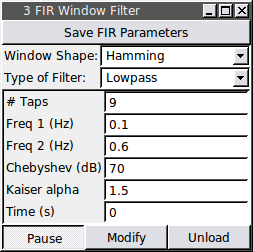
\includegraphics[width=2in]{FIRwindow.png} 
\caption[firfilter]{The wave maker module allows the output of a pre-recorded signal from an ASCII file.} 
\end{center}
\label{firfilter}
\end{figure}

The Finite Impulse Response Filter module creates an in-line FIR filter that can be applied to any signal in RTXI. Given the desired number of filter taps (filter order + 1), it computes the impulse response for a lowpass, highpass, bandpass, or bandstop filter using the window method. For a lowpass or highpass filter, the module uses the first frequency as the cut-off frequency. For a bandpass or bandstop filter, both input frequencies are used to define the frequency band. The module initially computes an ideal FIR filter to which you can apply a Triangular (or Bartlett), Hamming, Hann, Kaiser, or Dolph-Chebyshev window. The Hann window is not to be confused with the Hanning window (see MATLAB’s hann() vs. hanning() functions). To apply no window to the filter, choose the Rectangular filter. The Kaiser and Chebyshev windows each take a parameter that determines the attenuation of the sidelobes in the filter. The algorithms only accept an odd number of filter taps. If an even number is entered, the module will automatically add 1 to the number of filter taps.

\subsubsection{Input Channels}
\begin{description}
\item [Input]Signal to be filtered
\end{description}

\subsubsection{Output Channels}
\begin{description}
\item [Output]Filtered input signal
\end{description}

\subsubsection{Parameters}
\begin{description}
\item [Window Shape]  
  \begin{itemize}
  \item Rectangular
  \item Triangular (Bartlett)
  \item Hamming
  \item Hann
  \item Chebyshev
  \item Kaiser
  \end{itemize}
\item [Type of Filter]
  \begin{itemize}
  \item Highpass
  \item Lowpass
  \item Bandpass
  \item Bandstop
  \end{itemize}
\item [\# Taps]
\item [Freq 1 (Hz)]
\item [Chebyshev (dB)]
\item [Kaiser alpha]
\end{description}

\subsubsection{States}
\begin{description}
\item [Time (s)] Time elapsed, in seconds, since filter was started
\end{description}

\subsection{IIR Filter}
% IIR Filter Module

\subsubsection{Overview}
\label{IIR Filter}
\index{IIR Filter}\index{utilities, IIR Filter}\index{filter, IIR Filter}

\begin{figure}[h]
\begin{center}
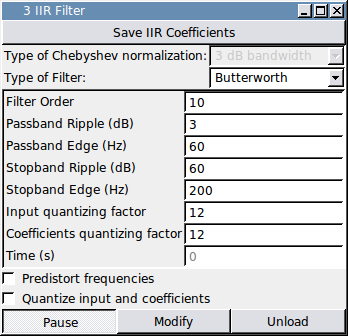
\includegraphics[width=3in]{IIRfilter.png}
\caption[iirfilter]{The infinite impulse response filter module can be used to filter  any signal in RTXI.}
\end{center}
\label{firfilter}
\end{figure}

This module computes coefficients for three types of filters. They require the following parameters:

Butterworth: passband edge
The Butterworth filter is the best compromise between attenuation and phase response. It has no ripple in the pass band or the stop band, and because of this is sometimes called a maximally flat filter. The Butterworth filter achieves its flatness at the expense of a relatively wide transition region from pass band to stop band, with average transient characteristics.

Chebyshev: passband ripple, passband edge
The Chebyshev filter has a smaller transition region than the same-order Butterworth filter, at the expense of ripples in its pass band. The filter minimizes the height of the maximum ripple. If you use a Chebyshev filter, you should also choose the type of normalization to apply.

Elliptical: passband ripple, stopband ripple, passband edge, stopband edge
An Elliptical (Cauer) filter has a shorter transition region than the Chebyshev filter because it allows ripples in both the stop and pass bands, giving a much higher rate of attenuation in the stop band. Elliptical filters give better frequency discrimination, but have a degraded transient response.

You may save the computed coefficients and the filter’s parameters to a file.

\subsubsection{Input Channels}
\begin{description}
\item [Input]Signal to be filtered
\end{description}

\subsubsection{Output Channels}
\begin{description}
\item [Output]Filtered input signal
\end{description}

\subsubsection{Parameters}
\begin{description}
\item [Filter order]An integer for the desired order for the filter
\item [Passband Ripple (dB)]
\item [Passband Edge (Hz)]
\item [Stopband Ripple (dB)]
\item [Stopband Edge (Hz)]
\item [Input quantizing factor]The number of bits to quantize the input signal to
\item [Coefficients quantizing factor]The number of bits to quantize the filter coefficients to
\end{description}

\subsubsection{States}
\begin{description}
\item [Time (s)] Time elapsed, in seconds, since filter was started
\end{description}

% Patch Clamp Experimental Suite
\clearpage
\section{Patch Clamp Experimental Suite}
The patch clamp experimental suite is a group of modules designed to aid an electrophysiologist during patch clamping. The suite includes modules for interfacing with patch clamp amplifiers, monitoring electrode resistance during gigaseal formation, and running voltage clamp experiments.

\subsection{Amplifier Control Modules}
The amplifier control modules are designed to easily interface RTXI with several common patch clamp amplifiers. These modules adjust scaling factors to compensate for amplifier gains based on the amplifier's current settings. Depending on the capabilities of the amplifier, the module may also have additional features, such as software controlled mode changing.

\subsubsection{AM Systems Model 2400}
\input{./utilities/am2400}

\subsubsection{Axon Axopatch 1-D}
\label{axon1dcommander}

\begin{figure}[h]
\begin{center}
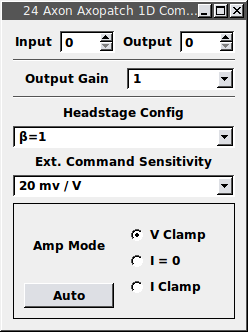
\includegraphics[width=2in]{axon1d.png}
\caption[axon1d]{The Axon Axopatch 1D Commander.}
\end{center}
\end{figure}

The settings of the module must match the settings of the Output Gain, Headstage Config, Ext. Command Sensitivity, and mode set by the amplifier's switches. The module is able to accept the amplifier's Gain Telegraph, allowing it to sense changes to the gain knob of the amplifier. It is also able to sense the mode of the amplifier through its Mode Telegraph. These are both located on the back of the amplifier.

input(0) - "Mode Telegraph" : The analog voltage signal from the amplifier's mode telegraph, allowing the module to determine the mode of the amplifier when the auto button is toggled

input(1) - "Gain Telegraph" : The analog voltage signal from the amplifier's gain telegraph, allowing the module to determine the gain set when the auto button is toggled.

\subsubsection{Axon Axopatch 200 Series}
\label{axon200commander}

\begin{figure}[h]
\begin{center}
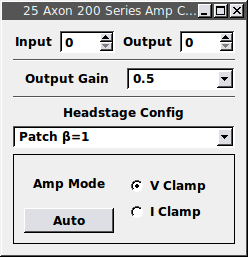
\includegraphics[width=2in]{axon200.png}
\caption[axon200]{Control module for Axon 200 Series Amplifier Commander.}
\end{center}
\end{figure}

Tested with the 200A and 200B, the Output Gain, Headstage Config, and Amp Mode must match the amplifier settings set by its switches. The module is able to sense the mode through the amplifier's mode telegraph, located on the back of the amplifier.

input(0) - "Mode Telegraph" : The analog voltage signal from the amplifier corresponding to the mode of the amplifier.

\subsubsection{Axon Multiclamp 700 Series}
\label{axon700commander}

\begin{figure}[h]
\begin{center}
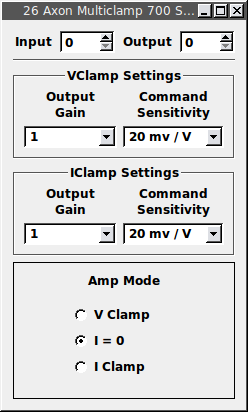
\includegraphics[width=2in]{axon700.png}
\caption[axon700]{This is the control module for Axon Multiclamp 700 Series Commander.}
\end{center}
\end{figure}

The VClamp and IClamp settings of the module must match the amplifier settings set by the user through the Axon software. The mode must also correspond to Axon software, unless the module is being to control the mode. Mode control is done through the amplifier's mode input located on the front of the amplifier.

output(0) - "Mode Telegraph" : Outputs an analog voltage signal to the amplifier through the mode telegraph, allowing the module to control the mode of the amplifier. The "Ext" box must be checked on the Axon software, located next to the mode.

\subsection{Membrane Test}
\input{./utilities/membranetest}

\subsection{Clamp Protocol}
\input{./utilities/clampprotocol}